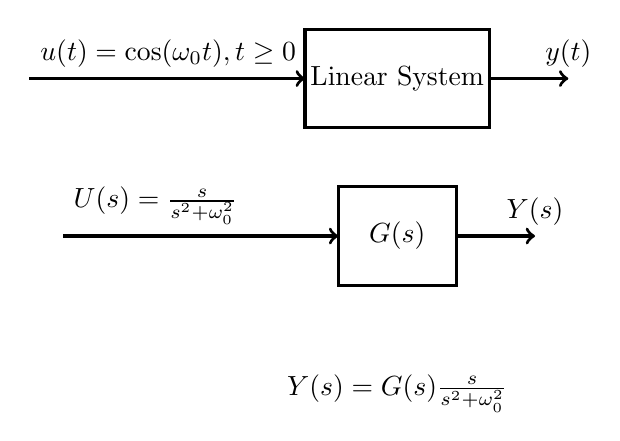
\begin{tikzpicture}[inner sep=0pt,outer sep=0pt,very thick,
sysblock/.style={draw,rectangle,inner sep=2pt,minimum width=1.5cm,minimum height=1.25cm,very thick}]
\draw (0,2) node[sysblock] (G1) {Linear System};
\draw[<-] (G1.180) -- ++(-3.5,0) node[above right=4pt] {$u(t) = \cos(\omega_{0}t), t \geq 0$};
\draw[->] (G1.0) -- ++(1,0) node[above=4pt] {$y(t)$};


\draw (0,0) node[sysblock] (G) {$G(s)$};
\draw[<-] (G.180) -- ++(-3.5,0) node[above right=4pt] {$U(s)=\frac{s}{s^{2}+\omega_{0}^{2}}$};
\draw[->] (G.0) -- ++(1,0) node[above=4pt] {$Y(s)$};

\draw (0,-2) node {$Y(s) = G(s)\frac{s}{s^{2}+\omega_{0}^{2}}$};
\end{tikzpicture}
